\subsection{Phases of matter}

An important area of research is the study of the different phases of (quantum) matter. A phase is a state
of matter in which the macroscopic physical properties of the substance are uniform on a macroscopic length scale. These phase can be measured by thermodynamic function, i.e. by function of a few macroscopic parameters. \cite{Nishimori2011}. More precisely, for a given phase the properties vary as an analytic function of the macroscopic variables.

Interesting physics happens at the boundary between 2 or more distinc phases. The phase transitions were classified by Ehrenfest \cite{Jaeger1998}, who looked at the free energy across the phase boundary. If the free energy shows a discontinuity, it is called first order (or discontinuous) phase transition. Similarly, if the derivitive shows a discontinuity, it is called second order (or continuous). Higher order phase transitions are possible, and there are even examples of infinite order transitions, such as the BKT transition.

\subsection{symmetry breaking}

Sometimes, but not always, a phase transition is  related to spontaneous symmetry breaking. A state $\ket{\Psi}$ is said to be symmetric under a unitary transformation U if the state only changes by a phase factor: $ \hat{U} \ket{\Psi} = e^{i \phi} \ket{\Psi} $. A hamiltonian posesses a symmetry if it commutes with U: $ [H,U]=0$  \cite{Beekman2019}. A remarkable fact is that many ground states are not invariant under a symmetry U of the hamiltonian.

For phase transitions associated with a broken symmetry, one can define an order parameter. This parameter evalutes to 0 for the symmetric phase, but not for the sponteous broken phase.

In continuous or second-order phase transitions the order parameter increases continuously from zero as the critical temperature is traversed. The entropy also changes continuously. On the other hand, the correlation length and related energy scales diverge at the critical temperature. In fact, at the critical temperature of a second-order phase transition, scale invariance systems become scale-invariant, in the sense that physical properties no longer depend on the length (or energy) scale at which they are probed. Many symmetry-breaking phase transitions are second-order, with the onsets of superfluidity, (anti)ferromagnetism and many phases of liquid crystals as famous examples.\cite{Beekman2019}

\subsection{Universality}

Universality looks at the behaviour of the system near a continuous phase transition. These can be discribed well by so called power laws. For classical phase transitions (driven by temperature) near critical temperature $T_c$, observables $a_i$ depend in the following way on the reduced temperature $t=\frac{T-T_c}{T_c}$: $ a_i(t) \sim t^{\alpha_i}$. One would expect that the set of critical exponents ${\alpha_i}$ depends on the precise form of the hamiltonian of the system, but it turns out these exponents can be captured by a limited numer of universality classes. This means that the physics near criticality is completely understood once it is understood for one member of the class.

\subsection{Critical exponents for spin systems}
The following table defines some of the critical exponents for the Ising system.

\begin{table}[h!]
    \centering
    \begin{tabular}{c c c c}
        Symbol & name                \\
        \hline
        m      & magnetisation       \\
        $\xi$  & correlation length  \\
        g      & external field      \\
        t      & reduced temperature \\
        d      & dimension           \\
    \end{tabular}
\end{table}

The 2 point correlation function is defined as $ f( x,y) =  \left < m(x) m(y) \right > -  \left<m(x) \right> \left<m(y) \right> $. At larger distances this decays exponentially fast (see \cref{crt:cft} ) $ f(  x,y ) = e^{ -\frac{ |x-y|}{ \xi} } $, where $\xi$ is the correlation length.

for the ordered phase, the following relations hold: $m ~ |t|^{\beta} $ , $\xi(t) \approx |t|^{-\nu} $. At the critical temperature near a quantum phase transition  $ m \approx |g-g_c|^{\frac{1}{\delta}} $.

\subsection{Finite size scaling}\label{subsec:fss}

Phase transitions only occur for systems with an infinite number degrees of freedom. This poses a problem, as in for instance Monte Carlo simulations only finite grids can be simulated. One computational expensive way to extract the properties in the thermodynamic limit is by making the grid increasingly bigger untill the properties have converged. Fisher's insight was that the properties could also be extrapolated from different finite size calculations by making the following assumption: near a critical point, every thermodynamic properties scales as an universal function of $L/\xi$, with L the size of the system and $\xi$ the correlation length.

Define $t=\frac{T-T_c}{T_c}$. The mathematical formulation is as follows:
\begin{equation}\label{eq:fssansatz}
    A(T,L) = L^{\kappa / \nu} f_A( t L ^{1/ \nu} )
\end{equation}
This holds for t small (near critical point) and L sufficient large compared to the lattice spacing. The exponents can be fitted by plotting $A(T,L)  L^{-\kappa / \nu} $ as a function of $t L ^{1/ \nu}$ for different sizes L and temperature t. For the correct critical exponents and critical temperature, all the points should collapse to one single graph.

From the ansatz \cref{eq:fssansatz}, other ways can be derived to determine certain coefficients.

\subsubsection{Finite size scaling for MPS}

The finite size scaling for MPS is somewhat different. In \cite{Vanhecke2019}, it is argued that $\delta$ can take the place of $1/L$.

Suppose $\lambda_i$ are the eigenvalues of \cref{vumps_transfer_eigs} order from largest real part to smallest. Then
\begin{equation}
    \epsilon_i = - \log( \left | \lambda_i  \right |  )
\end{equation}
Then
\begin{equation}
    \delta = - \sum_i c_i \epsilon_i
\end{equation}
The intuition behind this is as follows: for a MPS approximation, the gaps in the transfer spectrum go always to zero for sufficient large bond dimension. The distance between these gaps is thus a measure for the system size.

\subsubsection{subleading corrections}
In \cite{Beach2005}, it is argued that the form proposed in \cref{eq:fssansatz} does also not fully take into account the finite size effects. Subleading correction could be introduced as follows:
\begin{equation}
    A(T,L) = L^{\kappa / \nu} ( 1+c L^{-\omega} ) f_A( t L ^{1/ \nu} -d L^{-phi/nu} )
\end{equation}
Indeed, this reduces to \cref{eq:fssansatz} for sufficient large L. Because there is always data need around the critical point, the original procedure could be biased and result in wrong parameters. On the other hand, introducing extra parameters can lead to overfitting, again not improving the result.

\subsection{CFT}\label{crit:cft}

\todo{central charge}

\subsection{Quantum phase transitions}

A traditional 2nd order phase transition is driven by a change in temperature. Quantum phase transitions on the other hand happen at zero temperature under influence of another parameter g of the model. At finite temperature, 2 things can happen: either there is a line connecting a classical 2nd order phase transition to the quantum phase transition, or the phase transition disappears at finite temperature \cite{Sachdev1999}.

\begin{figure}
    \center
    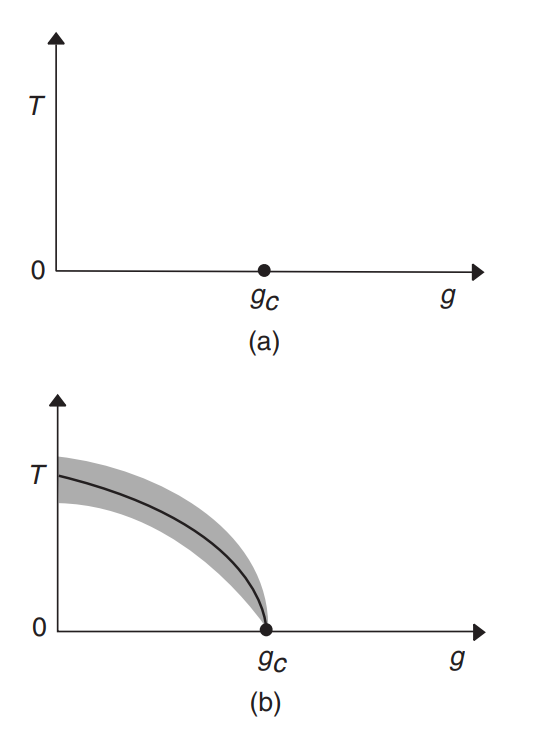
\includegraphics[width=0.5\textwidth]{Figuren/crit/Screenshot from 2021-05-06 15-58-55.png}
    \caption{ Two possible phase diagrams of a system near a quantum phase transition. In both cases there is a quantum critical point at $g = g_c$ and $T = 0$ . In (b), there is a line of $T > 0$ second-order phase transitions terminating at the quantum critical point. The theory of phase transitions in classical systems driven by thermal fluctuations can be applied within the shaded region of (b).  Figure and caption taken from \cite{Sachdev1999}. }
    \label{fig:crit:qtran}
\end{figure}

\subsection{Quantum to classical mapping}

\todo{Quantum to classical mapping}